\section{Every Claim Is a Command}
\label{sec:measured}

A recurring failure of educational material is the unmeasured claim (``MLA
saves memory''). In BabyWhale each module's payoff beat is a runnable script;
the figures below are plotted from the \emph{same numbers those scripts
print}, so a reader can reproduce every curve with one command.

\begin{figure}[t]
  \centering
  % Figure 2: two stacked ablation panels (data = what the course scripts print)
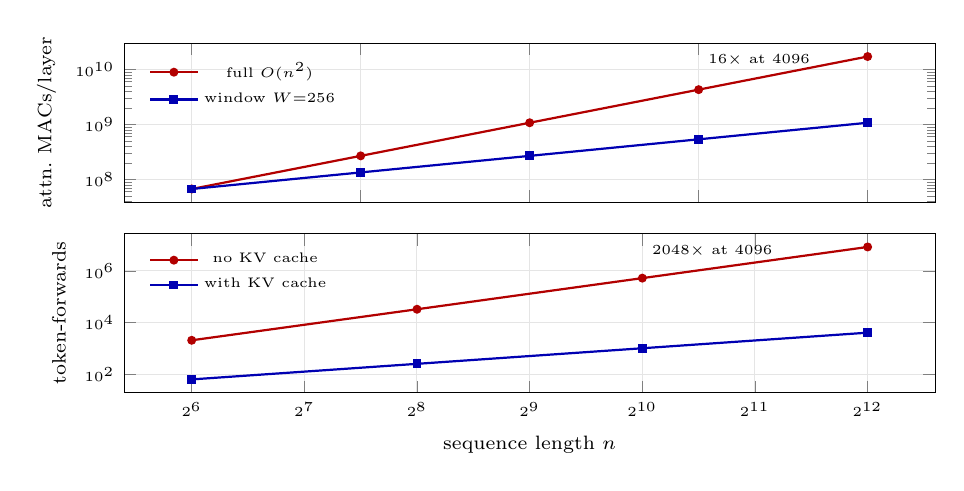
\begin{tikzpicture}
\begin{axis}[
  name=attn,
  width=0.98\columnwidth, height=3.6cm,
  xmode=log, ymode=log, log basis x=2,
  xlabel={}, ylabel={attn.\ MACs/layer},
  xticklabels={},
  legend style={font=\tiny, at={(0.02,0.95)}, anchor=north west, draw=none, fill=none},
  tick label style={font=\tiny}, label style={font=\scriptsize},
  grid=major, grid style={gray!20},
]
\addplot[color=red!70!black, mark=*, mark size=1.2pt, thick]
  coordinates {(256,67108864)(512,268435456)(1024,1073741824)(2048,4294967296)(4096,17179869184)};
\addlegendentry{full $O(n^2)$}
\addplot[color=blue!70!black, mark=square*, mark size=1.2pt, thick]
  coordinates {(256,67108864)(512,134217728)(1024,268435456)(2048,536870912)(4096,1073741824)};
\addlegendentry{window $W{=}256$}
\node[font=\tiny, anchor=west] at (axis cs:2048,15000000000) {$16\times$ at 4096};
\end{axis}
\begin{axis}[
  at={(attn.south west)}, anchor=north west, yshift=-4mm,
  width=0.98\columnwidth, height=3.6cm,
  xmode=log, ymode=log, log basis x=2,
  xlabel={sequence length $n$}, ylabel={token-forwards},
  legend style={font=\tiny, at={(0.02,0.95)}, anchor=north west, draw=none, fill=none},
  tick label style={font=\tiny}, label style={font=\scriptsize},
  grid=major, grid style={gray!20},
]
\addplot[color=red!70!black, mark=*, mark size=1.2pt, thick]
  coordinates {(64,2080)(256,32896)(1024,524800)(4096,8390656)};
\addlegendentry{no KV cache}
\addplot[color=blue!70!black, mark=square*, mark size=1.2pt, thick]
  coordinates {(64,64)(256,256)(1024,1024)(4096,4096)};
\addlegendentry{with KV cache}
\node[font=\tiny, anchor=west] at (axis cs:1024,6000000) {$2048\times$ at 4096};
\end{axis}
\end{tikzpicture}

  \caption{\textbf{Two of the six built-in ablations} (values as printed by
  \texttt{course/.../ablation.py}). \emph{Top:} per-layer attention MACs,
  full vs.\ a 256-token sliding window ($d{=}512$)---the quadratic/linear
  split that motivates windowed and compressed attention (Modules 02/04).
  \emph{Bottom:} token-forwards to generate $n$ tokens with and without a KV
  cache---the $O(n^2)\!\to\!O(n)$ decode saving (Module 14) reaches
  $2048\times$ at $n{=}4096$.}
  \label{fig:ablations}
\end{figure}

\paragraph{Analytic ablations.} Figure~\ref{fig:ablations} shows two of the
six: attention cost scaling and the KV-cache decode saving. The others print
the MLA cache footprint (MHA $2048$\,B vs.\ MLA $256$\,B per token per layer
at 8 heads $\times$ 128 dims, bf16: $8\times$ smaller at MQA size), MoE's
decoupling ($8\times$ parameters at $2\times$ FLOPs for 8 experts, top-2),
expected speculative tokens per verify pass ($4.1\times$ at draft-acceptance
$p{=}0.9$, $k{=}4$), and bf16$\to$FP4 weight memory ($4\times$).

\begin{figure}[t]
  \centering
  % Figure 3: the real reference pre-training run (BPE_REPORT curve, verbatim)
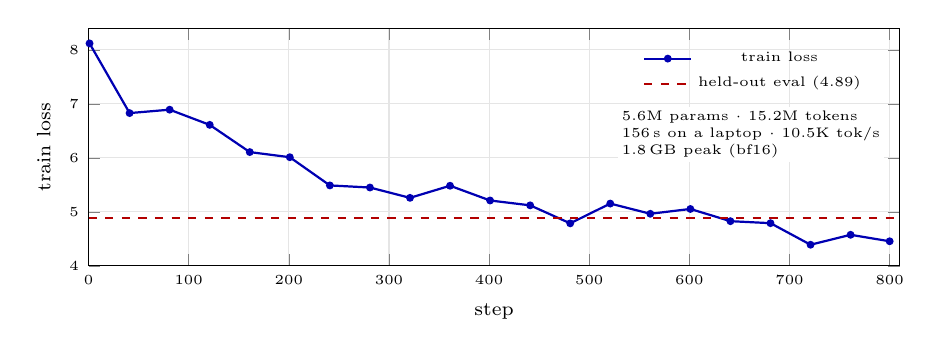
\begin{tikzpicture}
\begin{axis}[
  width=0.98\columnwidth, height=4.6cm,
  xlabel={step}, ylabel={train loss},
  xmin=0, xmax=810, ymin=4, ymax=8.4,
  tick label style={font=\tiny}, label style={font=\scriptsize},
  legend style={font=\tiny, draw=none, fill=none, at={(0.97,0.95)}, anchor=north east},
  grid=major, grid style={gray!20},
]
\addplot[color=blue!70!black, thick, mark=*, mark size=1pt]
  coordinates {(1,8.119)(41,6.829)(81,6.892)(121,6.611)(161,6.107)(201,6.012)
               (241,5.490)(281,5.451)(321,5.260)(361,5.484)(401,5.211)(441,5.121)
               (481,4.788)(521,5.154)(561,4.965)(601,5.054)(641,4.828)(681,4.791)
               (721,4.392)(761,4.576)(800,4.456)};
\addlegendentry{train loss}
\addplot[color=red!70!black, dashed, thick] coordinates {(0,4.886)(810,4.886)};
\addlegendentry{held-out eval (4.89)}
\node[font=\tiny, align=left, anchor=north east, fill=white, inner sep=1.5pt]
  at (axis cs:795,6.95)
  {5.6M params $\cdot$ 15.2M tokens\\ 156\,s on a laptop $\cdot$ 10.5K tok/s\\ 1.8\,GB peak (bf16)};
\end{axis}
\end{tikzpicture}

  \caption{\textbf{The lifecycle actually runs on a laptop.} Training loss of
  the course's reference pre-training run: a 5.6M-parameter model (2048-token
  BPE vocabulary) over 15.2M tokens---800 steps in 156\,s on an Apple-Silicon
  laptop ($\sim$10.5K tok/s, 1.8\,GB peak, bf16). Held-out evaluation loss
  4.89 (dashed). The same checkpoint then proceeds through mid-training,
  SFT, DPO, RL, quantization, and serving in the course.}
  \label{fig:loss}
\end{figure}

\paragraph{A real end-to-end run.} Figure~\ref{fig:loss} shows the course's
reference pre-training run, produced by the repository's own CLI on consumer
hardware. Laptop-scale matters pedagogically: every stage of the lifecycle,
including the RL loop and the batching server, completes in classroom time,
so ``break it and re-run'' is a five-minute experiment rather than a cluster
job. The fast byte-BPE encoder this run depends on is itself a course story:
the naive encoder stalls on long lines, while the heap-based one packs the
15.2M-token corpus in 52\,s---and the corresponding lab requires the
learner's simple encoder to match it token-for-token.

\paragraph{Continuous verification.} All of the above---334 tests, the two
auto-gated milestones, the drift and coverage guards, and a strict
documentation build---run in public CI on Apple-Silicon runners; the course
site is redeployed on every push to \texttt{main}.
